% File: thesis/figures/fig_3_16_lcoh_cashflow.tex
\documentclass[tikz,border=10pt]{standalone}
\usepackage{tikz}
\usepackage{amsmath}
\usepackage{amssymb}
\usepackage{pgfplots}
\pgfplotsset{compat=1.18}
\usetikzlibrary{
    arrows.meta, 
    positioning, 
    calc,
    patterns,
    decorations.pathmorphing,
    backgrounds,
    shadows
}

% Colors
\definecolor{capexcolor}{RGB}{52,103,81}      % Dark green - investment
\definecolor{opexcolor}{RGB}{86,160,211}      % Blue - operating
\definecolor{discountcolor}{RGB}{200,82,45}    % Orange - decay
\definecolor{resultcolor}{RGB}{162,59,114}     % Purple - final LCOH
\definecolor{energycolor}{RGB}{218,165,32}     % Gold - energy delivered

\begin{document}
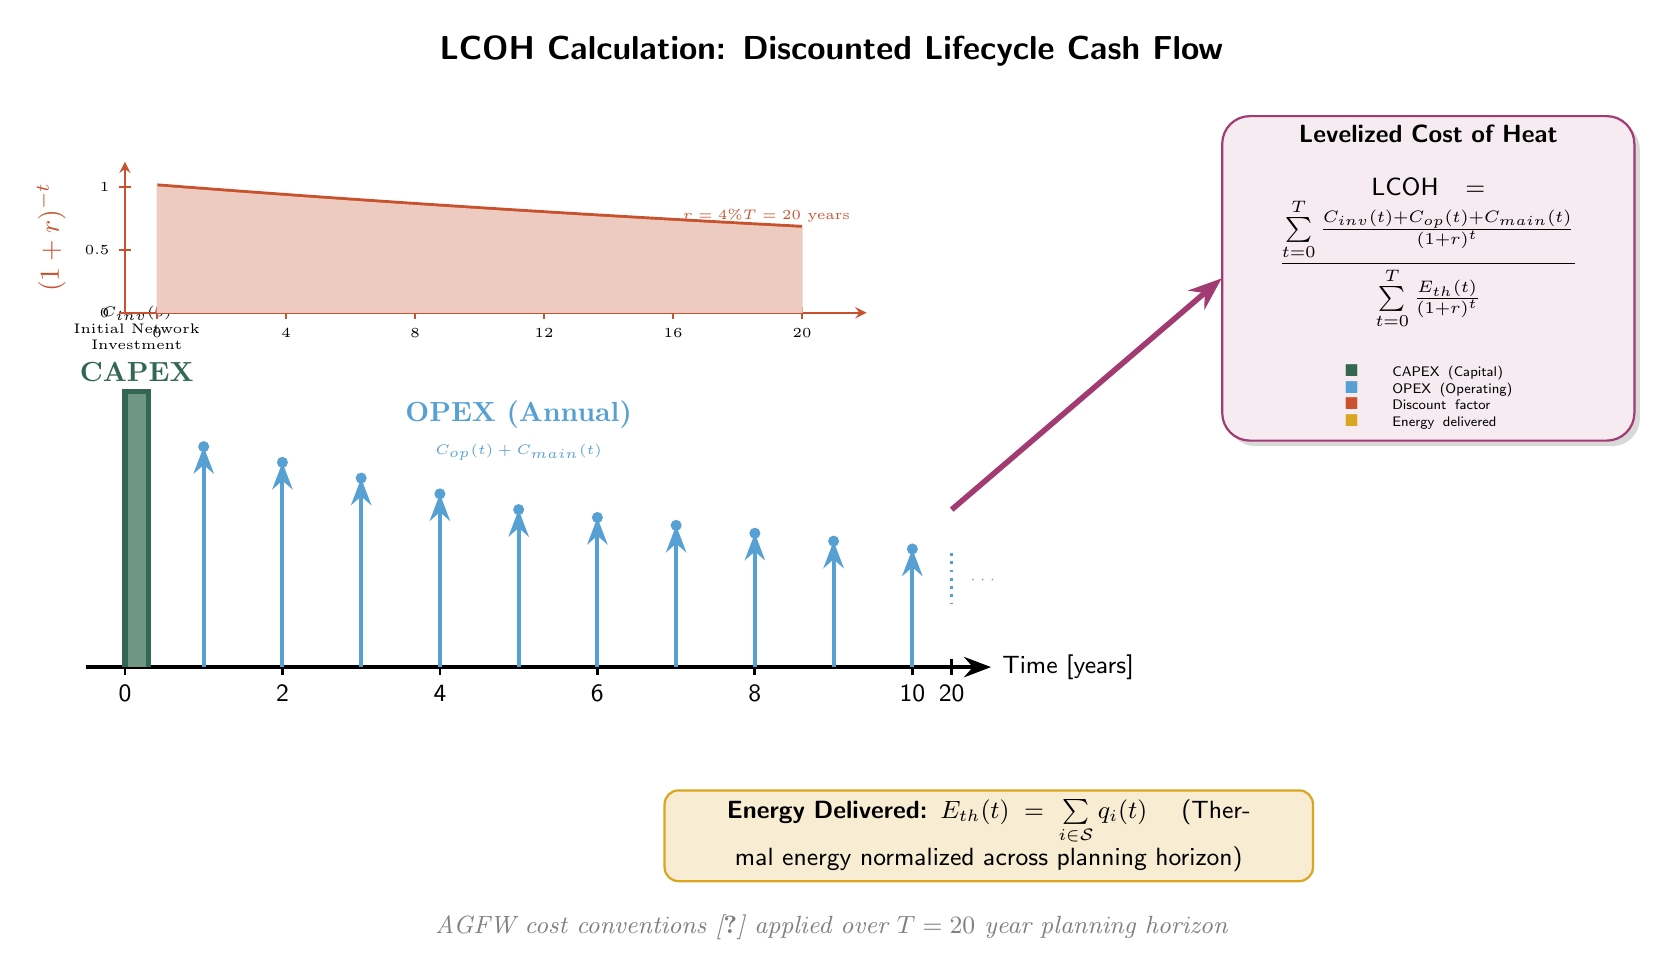
\begin{tikzpicture}[
    font=\small\sffamily,
    >=Stealth,
    thick
]

% === TIMELINE AXIS ===
\draw[->, line width=1.5pt] (-0.5,0) -- (11,0) node[right] {Time [years]};
\foreach \x in {0,2,4,6,8,10} {
    \draw[line width=1pt] (\x,0.1) -- (\x,-0.1) node[below] {\x};
}
\draw[line width=1pt] (10.5,0.1) -- (10.5,-0.1) node[below] {20};

% === CAPEX BAR (Year 0) ===
\fill[capexcolor!70] (0,0) rectangle (0.3,3.5);
\draw[capexcolor, line width=2pt] (0,0) -- (0,3.5) -- (0.3,3.5) -- (0.3,0);
\node[above, font=\bfseries, capexcolor] at (0.15,3.5) {CAPEX};
\node[above=0.2cm, font=\tiny, align=center] at (0.15,3.7) {
    $C_{inv}(0)$\\
    Initial Network\\
    Investment
};

% === OPEX ARROWS (Annual) ===
% Show arrows for years 1-20 with decreasing height (simplified)
\foreach \year/\height in {1/2.8, 2/2.6, 3/2.4, 4/2.2, 5/2.0, 6/1.9, 7/1.8, 8/1.7, 9/1.6, 10/1.5} {
    \draw[->, opexcolor, line width=1.5pt] (\year,0) -- (\year,\height);
    \fill[opexcolor] (\year,\height) circle (2pt);
}
% Dotted line for continuation
\draw[opexcolor, dotted, line width=1pt] (10.5,1.45) -- (10.5,0.8);
\node[opexcolor, font=\tiny, right] at (10.6,1.1) {$\cdots$};

% Label for OPEX
\node[above=0.3cm, font=\bfseries, opexcolor, align=center] at (5,2.2) {
    OPEX (Annual)\\
    \tiny$C_{op}(t) + C_{main}(t)$
};

% === DISCOUNT CURVE ===
\begin{axis}[
    at={(0cm, 4.5cm)},
    anchor=south west,
    width=11cm,
    height=3.5cm,
    xtick={0,2,4,6,8,10},
    xticklabels={0,4,8,12,16,20},
    ytick={0,0.5,1},
    yticklabels={0,0.5,1},
    xmin=-0.5, xmax=11,
    ymin=0, ymax=1.2,
    axis lines=left,
    xlabel={},
    ylabel={$(1+r)^{-t}$},
    ylabel style={font=\small, discountcolor, font=\bfseries},
    tick label style={font=\tiny},
    axis line style={thick, discountcolor},
    y axis line style={thick, discountcolor},
    every tick/.style={thick, discountcolor},
]

% Discount curve (1+r)^-t with r=0.04
\addplot[discountcolor, line width=2.5pt, domain=0:10, samples=100] 
    {exp(-0.04*x)};
\addplot[discountcolor!30, fill, domain=0:10, samples=100] 
    {exp(-0.04*x)} \closedcycle;

% Annotation for discount rate
\node[anchor=north west, font=\tiny, discountcolor] at (axis cs:8,0.9) {
    $r = 4\%$\\
    $T = 20$ years
};

\end{axis}

% === LCOH FORMULA BOX (Right side) ===
\node[
    rectangle,
    rounded corners=10pt,
    draw=resultcolor,
    fill=resultcolor!10,
    text width=5cm,
    minimum height=3.5cm,
    align=center,
    right=1cm of current bounding box.east,
    yshift=2cm,
    drop shadow={shadow xshift=2pt, shadow yshift=-2pt, opacity=0.3}
] (lcohbox) {%
    \textbf{Levelized Cost of Heat}\\[8pt]
    $\text{LCOH} = \dfrac{\sum\limits_{t=0}^{T} \frac{C_{inv}(t) + C_{op}(t) + C_{main}(t)}{(1+r)^t}}{\sum\limits_{t=0}^{T} \frac{E_{th}(t)}{(1+r)^t}}$\\[12pt]
    \tiny
    \begin{tabular}{ll}
    \textcolor{capexcolor}{$\blacksquare$} & CAPEX (Capital) \\
    \textcolor{opexcolor}{$\blacksquare$} & OPEX (Operating) \\
    \textcolor{discountcolor}{$\blacksquare$} & Discount factor \\
    \textcolor{energycolor}{$\blacksquare$} & Energy delivered
    \end{tabular}
};

% Arrow pointing to formula
\draw[->, line width=2pt, resultcolor] (10.5,2) -- (lcohbox.west);

% === ENERGY DELIVERED (Bottom - denominator visualization) ===
\node[
    rectangle,
    rounded corners=5pt,
    draw=energycolor,
    fill=energycolor!20,
    text width=8cm,
    minimum height=1cm,
    align=center,
    below=1cm of current bounding box.south,
    xshift=2cm
] (energybox) {%
    \textbf{Energy Delivered:} $E_{th}(t) = \sum\limits_{i \in \mathcal{S}} q_i(t)$ \quad
    (Thermal energy normalized across planning horizon)
};

% === ANNOTATIONS ===
\node[above=0.5cm, font=\large\bfseries\sffamily] at (current bounding box.north) {%
    LCOH Calculation: Discounted Lifecycle Cash Flow
};

\node[below=0.3cm, font=\small\itshape, text=gray] at (current bounding box.south) {%
    AGFW cost conventions \cite{AGFWFW401_2022} applied over $T = 20$ year planning horizon
};

\end{tikzpicture}
\end{document}
